% !TeX root = ../main.tex
% Add the above to each chapter to make compiling the PDF easier in some editors.

\chapter{Related Work}\label{chapter:Related Work}
In this section projects from third parties are going to be inspected, who also did work related to recognizing traffic signs, their used methods are pointed out, seeking to explain why they have been used.

\section{Computer Vision}
\subsection{OpenCV Based Road Sign Recognition on Zynq}\label{zynq}
\begin{figure}[H]
	\centering
	\minipage{0.6\textwidth}
	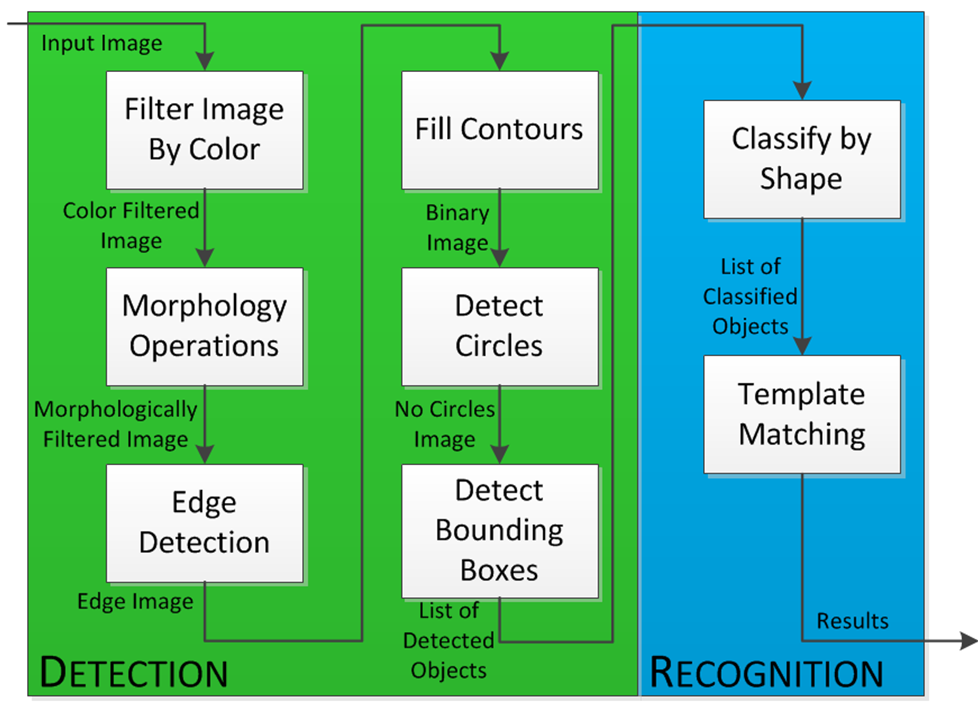
\includegraphics[width=\linewidth]{images/zynqconcept.png}
	\caption{Concept \cite{zynq}}\label{fig:zynq}
	\endminipage\hfill
\end{figure}
The paper by Matthew Russell and Scott Fischaber presents a system on chip approach with a Xilinx Zynq-7020 chip, for recognizing and classifying road signs. The methods for detection are color-based techniques paired with shape recognition, implemented with the OpenCV library. To finally classify the regions of interest, found in the first steps, template matching is used. The system's performance is around 0.2 frames per second \cite{zynq}. Subsequent paragraph is going to describe the methods used to extract certain regions, that might be important for the task of road sign detection, thus the green part of figure \ref{fig:zynq}. \newline
The first stage in the algorithm is
converting the image into the HSV color space, in order to remove background colors (Figure: \ref{fig:zynq0}). HSV was chosen over HSI, because it is easier to implement in hardware, calculating  HSI requires more divisions and would therefore increase latency in hardware, resulting in an overall slowed down system. With the focus on red and blue traffic signs, red and blue pixels are being extracted and thresholded by the algorithm (Figure: \ref{fig:zynq1}). Therafter Morphology  operations  are  applied  to  the  filtered image to recover some broken signs and to remove very small objects. After being converted to gray scale (Figure: \ref{fig:zynq2}), the Canny Edge detection is being used, to determine every edge in given image (Figure: \ref{fig:zynq3}), provided by OpenCV. Resulting picture is searched for contours, found contours are being filled with white pixels (Figure: \ref{fig:zynq4}), whereas contours smaller than 30 pixels are removed, the image is binary now. The next operation cuts every circle out of the picture (Figure: \ref{fig:zynq5}), to determine where circles are, the Circle Hough Transform from OpenCV is applied.
Another useful tool, provided by this library is the  Ramer-Douglas-Peucker 
algorithm, that is used to approximate a shape.
This is applied to the remaining filled contours, in order to count the number of corners. The count is used
to classify the shape as a triangle (3), rectangle(4), octagon(8) or unknown(others). This is repeated for all detected bounds and the detected shapes are joined with the list of circles to form a full list of detected sign candidates in the image. Mentioned list is now passed to the recognition step, where these nominees are classified via Template Matching. \newline
As the purpose of addressing this work, was to highlight the Computer Vision aspect, so the classification, the overview ends here, but more about the recognition can be read independently in the paper \cite{zynq}. 

\begin{figure}[H]
	\minipage{0.33\textwidth}
	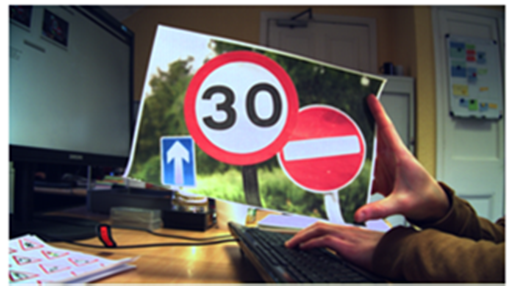
\includegraphics[width=\linewidth]{images/zynq0.png}
	\caption{HSV}\label{fig:zynq0}
	\endminipage\hfill
	\minipage{0.33\textwidth}
	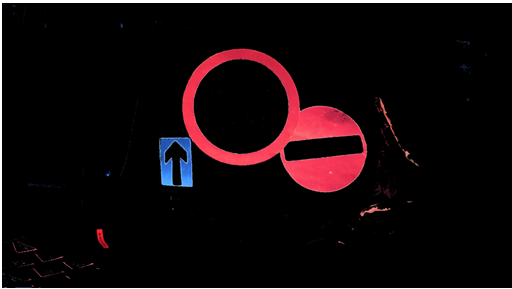
\includegraphics[width=\linewidth]{images/zynq1.png}
	\caption{Thresholded}\label{fig:zynq1}
	\endminipage\hfill
	\minipage{0.33\textwidth}%
	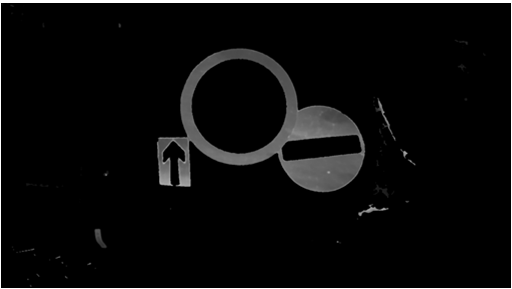
\includegraphics[width=\linewidth]{images/zynq2.png}
	\caption{Grayscale}\label{fig:zynq2}
	\endminipage\hfill
	\newline
	\minipage{0.33\textwidth}
	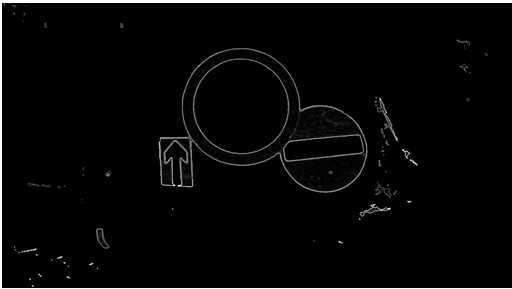
\includegraphics[width=\linewidth]{images/zynq3.png}
	\caption{Canny}\label{fig:zynq3}
	\endminipage\hfill
	\minipage{0.33\textwidth}
	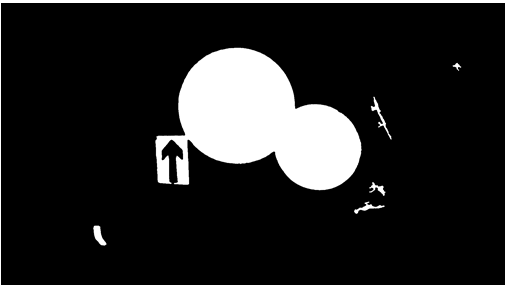
\includegraphics[width=\linewidth]{images/zynq4.png}
	\caption{Filled}\label{fig:zynq4}
	\endminipage\hfill
	\minipage{0.33\textwidth}%
	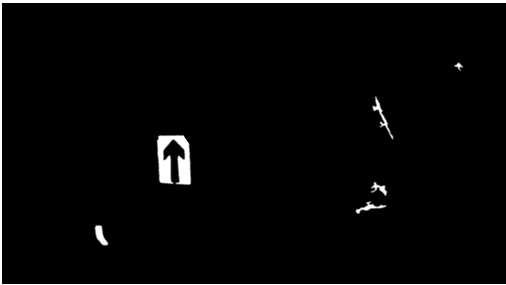
\includegraphics[width=\linewidth]{images/zynq5.png}
	\caption{Extracted}\label{fig:zynq5}
	\endminipage
	\newline
	\caption*{Steps of processing the image \cite{zynq}}
\end{figure}

\subsection{Other approaches}
Different computer vision based methods, are also imaginable in the field of traffic sign detection, more generalized there are two different methods: shape- and color based \cite{moglemose}. But just like in \ref{zynq} often Hybrid forms are created. An example used for shape based methods is the Histogram Of Oriented Gradients (HOG) \cite{hogex}, or the Hough Transform and it's derivatives. Color based filtering techniques are also wide spread, as the analysis from Andreas Møgelmose indicates \cite{moglemose}. 
It is also pointed out, each method has its pros and cons. While color based techniques might have a deficit in terms of changing lightning conditions, or bleached signs, due to erosion, algorithms targeting shapes, possibly have problems detecting partly covered signs. 


\section{Machine Learning}
\subsection{ICJNN}\label{ssec:machinelearning}

J. Stallkamp, M. Schlipsing, J. Salmen and C. Igel wrote their paper \cite{machinelearning}, in order to give a brief overview of the machine learning algorithms in the field of traffic sign recognition, with regard to the classification. \newline
They point out, that some subsets of classes are
very similar to each other (e.g., speed limit signs). In addition to these interclass differences and similarities, the classifier must be able to handle different optical appearances, like changes in lighting, partial occlusions, rotations and diverse other irregularities. In 2011 a competition named: "IEEE Joint
Conference on Neural Networks" (IJCNN) \footnote{\url{http://benchmark.ini.rub.de./} (visited on 02.14.2018)} took place, in order to compare pattern recognition and machine learning approaches. Over 20 participating teams competed against each other, with the following approaches: different kinds of neural
networks (NN), support vector machines (SVMs), linear discriminant analysis, subspace analysis, ensemble classifiers, slow feature analysis, nearest neighbor classifiers and random forests. \newline
The first and the second place were won by classifiers both using convolutional Nerual Networks, the third place was won by a random forest technique approach, paired with a Support Vector Machine. Notably, in the course of the competition, a human's performance on single framed image recognition was tested, as comparison, resulting in a score of 98.84\% correctly recognized images. In contrast to this result, the first place, utilizing a multi-column deep neural network (MCDNN) scored a total of 99.46\%, therefore beeing even better than a real person. 


\begin{table}[h]
	\begin{tabular}{||p{0.05\linewidth} | p{0.2\linewidth}|p{0.2\linewidth}|p{0.2\linewidth}|p{0.2\linewidth}||}
		\hline
		Rank  &	Team & Representative &	Method &	Correct recognition rate\\
		\hline
		\hline
		1 & IDSIA & Dan Ciresan & Committee of CNNs &	99.46\% \\
		\hline
		2 &	INI & & Human Performance & 98.84\% \\
		\hline
		3 & sermanet & Pierre Sermanet & Multi-Scale CNNs & 98.31 \% \\
		\hline
		4 & CAOR & Fatin Zaklouta & Random Forests &	96.14\% \\
		\hline
		
	\end{tabular}
	\caption{Final results of the IJCNN 2011}
	\label{table:icjnn2011}
	
\end{table}

\subsection{More traditional approaches}
There are numerous different methods to implement artificial intelligences, some of them are newer and some may have existed for a decent amount of time. 
A good example for older kinds of machine learning might be decision tree learning \cite{decision}, although in direct comparison to other techniques like deep learning, this projection might come off poorly, because decision trees tend to be inaccurate, besides they are not really robust. Small changes in data might cause a big difference in the final prediction \cite{decisionbook}. \newline
Support Vector Machines are another avenue, they often occur, in terms of image recognition. As could be seen in \ref{ssec:machinelearning}, this projection could not keep up with neural networks. Known limitations are the speed and size in training as well as testing, besides their algorithmic complexity and memory requirements in large-scale tasks are likely to be negative factors \cite{burges}. 


\section{Deep Learning}\label{ssec:koreancnn}


\if false

\subsection{Traffic Sign Recognition system on Android devices}
Another really good example of similar work, that has been produced on the topic of traffic sign recognition was done by Tran, Hai S., Traffic Sign Recognition was implemented on an Android device. This system was designed to recognize 85 New Zealand traffic signs with various colours and shapes \cite{androidnn}. \newline
Two different techniques are used to extract sign candidates from raw images before they are classified to the correct class. The first technique uses colour filters to specify relevant regions, as the
second technique applies the detector on two consecutive raw images without colour-filtering. As mentioned Sign detector an AdaBoost classifier using Linear Binary Pattern was utilized to extract required features. Regions of interest from the sign detector are called ”sign candidates” and classified by a back propagating neural network. 

\begin{figure}[H]
	\centering
	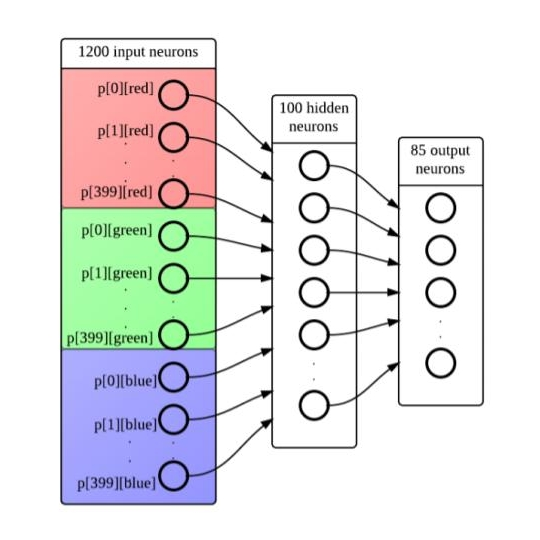
\includegraphics[height=5cm]{images/tranNN.jpg}
	\caption{Applied Neural Network}
	\label{fig:tranNN}
\end{figure}




This report
finds the colour-filtering technique with the filtering threshold carefully tuned
overperforms the cascade detecting technique, but the latter is less likely to
miss a sign in different lighting conditions.

\fi

\subsection{Real-time Traffic Sign Recognition System with Deep Convolutional Neural Network}
It should be mentioned, that convolutional neural networks (CNN) are frequently used, when it comes to classifying images.
In this subsection, the attention is on the classifying part of the project by Seokwoo Jung, Unghui Lee, Jiwon Jung and David Hyunchul Shim \cite{tsrcnn}. 
Their paper, describes a system, that is trained to classify six types of traffic signs by a convolutional
neural network architecture. In the detection phase, light-weight color-based segmentation and the Hough transform  are applied to extract sign candidates, that can be fed onwards into their CNN. The recognition system nearly achieves real-time performance, according to them. \newline
Every proposed region of interest is resized to a square format of 100 by 100 pixels, with an additional third dimension of three values, representing R, G and B. Their Output layer is designed to have eight nodes, although the system aims to differentiate between six distinguishable signs. The two additional neurons are for representing, whether the sign is a sign but none of the six wanted and to indicate, that a candidate is no sign at all. After each convolutional layer, the amount of data is being reduced.  
At first, the
training happened only with positive samples, created by hand cropped images. After several tests, false positive classifications have been collected (78000 samples), and reused to train the network again, mixed together with the positive images (25000). As camera input, a GoPro HERO 4 was connected to a PC running an i7-6820HK CPU and a Titan X graphic card with 12gb memory. As Neural Network framework Caffe has been used for implementation.

\begin{figure}[H]
	\centering
	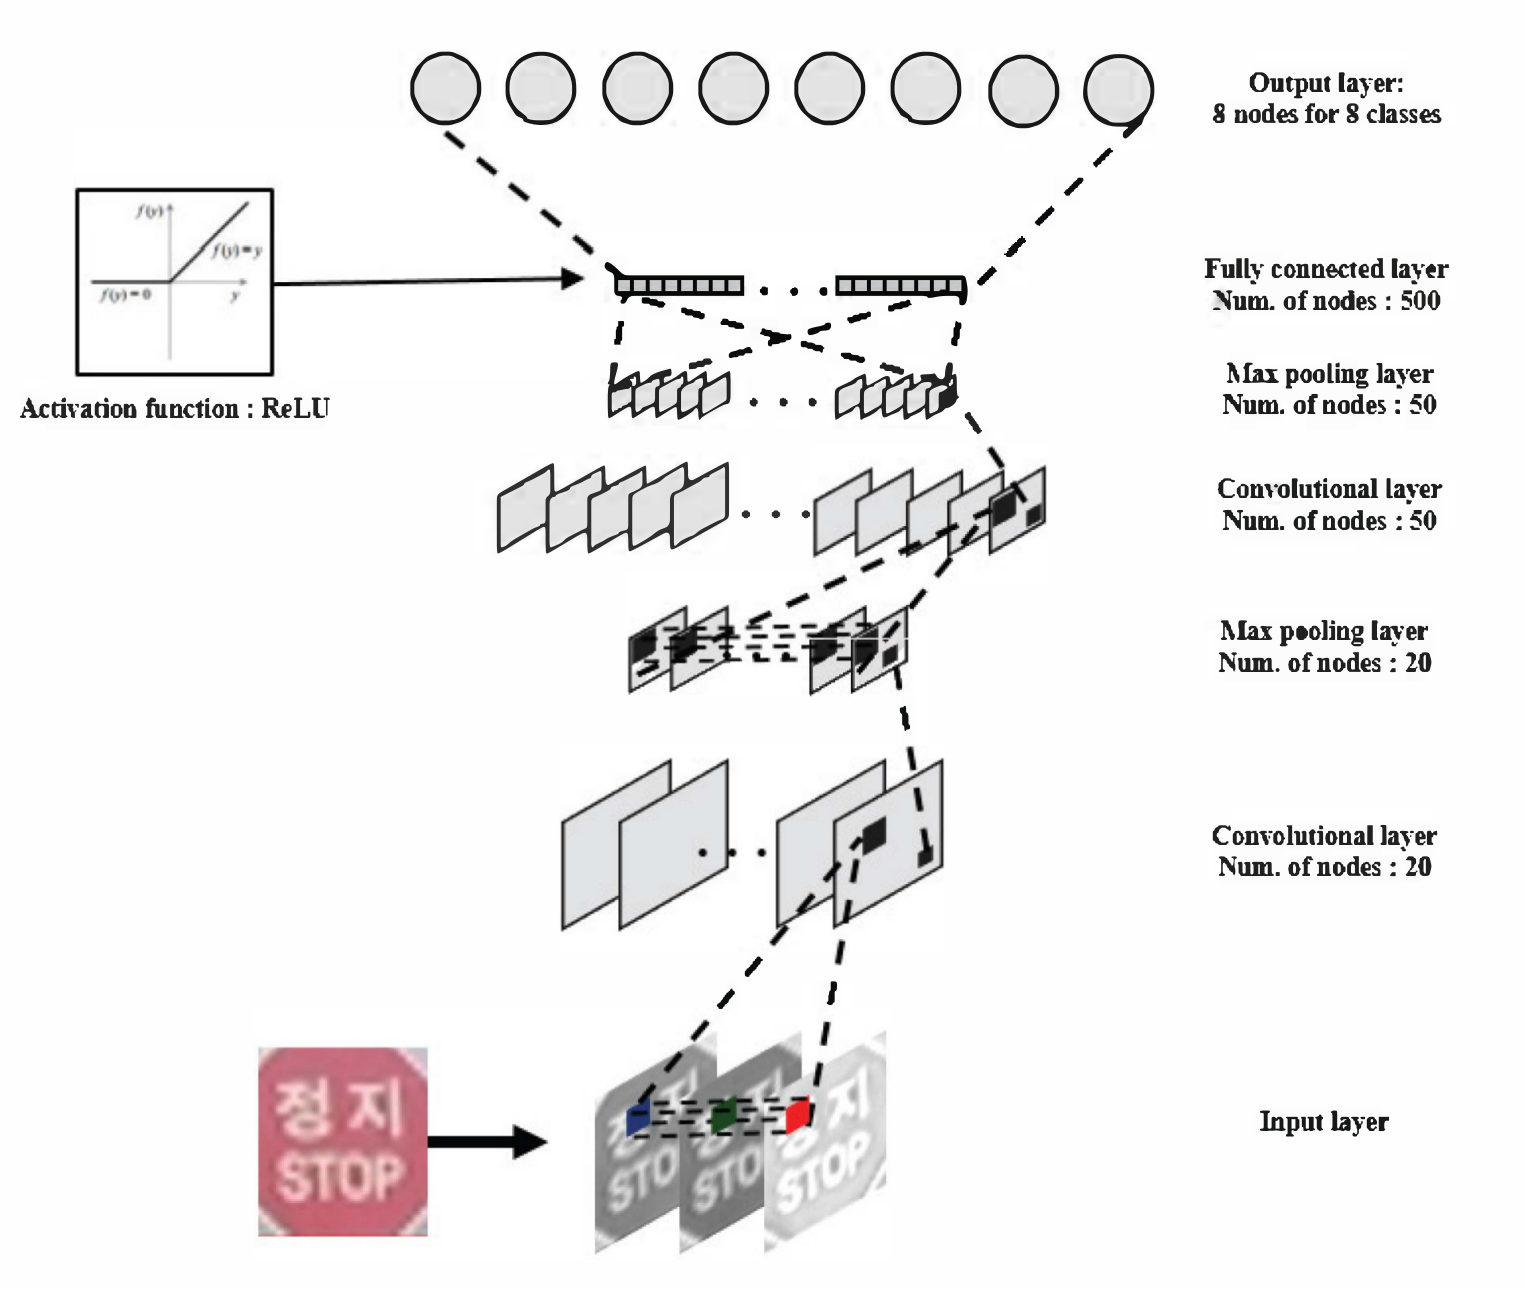
\includegraphics[width = 0.75\linewidth]{images/koreancnn.png}
	\caption{Applied Convolutional Neural Network \cite{tsrcnn}}
	\label{fig:koreanNN }
\end{figure}
\subsection{Common neural networks}
Though when the task is to classify an image, convolutional neural networks can be considered being state of the art right now, there are a lot of other kinds of networks, like autoencoder networks \cite{bengio}. However this special architecture aims to transform the input values, but keeps the format, therefore the input and output neurons have to be the same quantity. This makes the ANN unsuitable for tasks like classifications.\newline
Shallow ANN, only have one hidden Layer inside, nevertheless, they can also be used for tasks like classifying traffic signs. Tran, Hai S. ran such a network on an Android phone scoring a 84\% success rate on detecting the signs\cite{tran}. Considering there was only one hidden layer used with 100 neurons, this can actually be considered a pretty decent result.

\newpage
\section{Conclusion}
As from subsection \ref{ssec:machinelearning} emerges, artificial neural networks (ANN) play an important role in classifying images and their performance seems to be overwhelming, because these approaches are even capable of outperforming human image classification. So the direction for the following project was set towards a neural network based system. Though convolutional are often the architecture of choice, they require a decent amount of computing power provided by the hardware, like in subsection \ref{ssec:koreancnn}. Furthermore given the task of only classifying numbers, a more simple network, could also be sufficient. Regarding these aspects, the choice was made to utilize a deep but not convolutional ANN, with respect to the more or less minimalistic circumstances of using an Android powered device.